\section{Ondes sonores - le son }

\subsection{Trois caractéristiques du son}

Lorsque vous écoutez une mélodie jouée par un instrument de musique ou
une personne qui parle, vous pouvez déterminer de quel instrument il
s'agit ou quelle est la personne qui parle.

Vous pouvez également détecter les différences de fréquence et les
variations de volume sonore.

Le son a trois caractéristiques~:
\begin{enumerate}
   \item La hauteur~: liée à la fréquence. 
La hauteur du son est la sensation d'aigu ou de grave. Elle est liée à
la fréquence de vibration de la source oscillante.

Un son grave pour l'oreille humaine correspond à une basse fréquence, un
son aigu à une fréquence élevée.

L'oreille humaine perçoit des sons si leur fréquence est comprise
approximativement entre 16 Hz et 20 kHz.

D'un point de vue musical, la hauteur du son détermine la note.

\item Le timbre

Le timbre d'un son est la sensation physiologique qui permet de
distinguer deux sons de même fréquence mais dont la perception semble
différente. C'est une caractéristique du son qui nous permet de
déterminer la différence entre deux voix de deux personnes différentes.

\item L'intensité sonore.

C'est la caractéristique du son liée à l'amplitude du son perçu. Nous
disons dans le langage courant qu'il s'agit du volume du son (plus ou
moins «~fort~»).
\end{enumerate}

\subsection{Intensité sonore}

Une source sonore produit une onde qui est captée par un auditeur se
trouvant à une certaine distance de l'émetteur.

Quelle sera l'intensité sonore perçue par le capteur~? Comment définir
cette intensité sonore~?

\begin{figure}
\centering
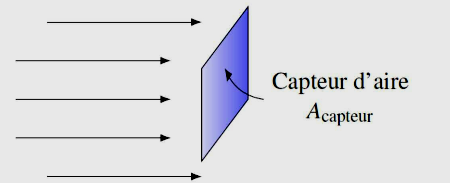
\includegraphics[width=6.442cm,height=2.623cm]{Pictures/10000001000001C2000000B7D5766B8618542229.png}
\caption{}
\end{figure}

\begin{enumerate}
\item Énergie captée en fonction de la surface du capteur

Dans le cas d'une onde sonore à une dimension, un capteur situé juste à
côté de l'émetteur reçoit la totalité de la puissance de l'onde, car
l'onde n'a pas d'autre place où aller.

\begin{figure}
\centering
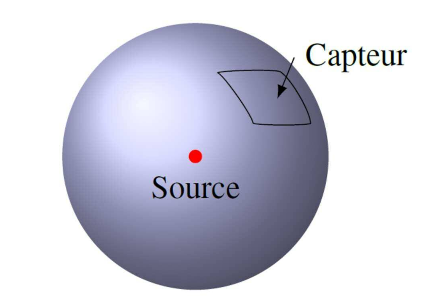
\includegraphics[width=5.355cm,height=3.808cm]{Pictures/10000001000001A50000012CD4D736604ADF8EAC.png}
\caption{}
\end{figure}

Pour une onde en trois dimensions (produisant un son de façon isotrope
dans toutes les directions), le capteur ne captera qu'une partie de
l'onde, car seule une partie de l'onde atteint le capteur. L'énergie
captée dépend donc de la surface du capteur.

\item Énergie captée en fonction du temps

Évidemment, on captera plus d'énergie si on capte l'énergie de l'onde
pendant plus de temps. La quantité d'énergie captée doit donc être
proportionnelle au temps pendant lequel on capte l'énergie.
\end{enumerate}

L'énergie captée (E)~ est~: 
\begin{itemize}
\item proportionnelle à un facteur qui va dépendre de l'énergie de l'onde.
On va appeler ce facteur \emph{l'intensité de l'onde (I).} On capte peu
d'énergie avec une onde de faible intensité et beaucoup avec une onde de
grande intensité. La quantité d'énergie captée doit donc être
proportionnelle à l'intensité $I$ de l'onde.
 \item proportionnelle à la surface du capteur (A)
 \item proportionnelle au temps durant lequel le capteur reçoit l'onde (t).
\end{itemize}

Donc, une bonne définition de l'intensité sonore est l'énergie
captée par unité de surface et de temps autrement dit la puissance
captée par unité de surface. 

L'intensité sonore s'exprime donc en \si{w/m^2}.

\subsection{Intensité sonore et échelle logarithmique}

L'oreille humaine peut capter des sons dont l'intensité est
au minimum de $10{-12}$ \si{w/m^2}.

Si le son a une intensité plus petite que cette valeur, on n'entend pas
le son.

L'intensité sonore minimale perceptible par l'oreille humaine est de
$10^{-12} \si{w/m^2}$.

Une conversation normale correspond à une intensité de
$3 10^{-6} \si{w/m^2}$.

Le son devient trop intense pour l'oreille humaine si son intensité
dépasse  $1 \si{W/m^2}$ approximativement. C'est le seuil de
la douleur.

Des bruits dangereux pour l'oreille correspondent à
$10^2 \si{W/m^2}$ et plus.

Une intensité sonore de $10^5 \si{w/m^2}$ serait l'intensité sonore perçue si vous placiez votre oreille à la
sortie d'un réacteur d'avion. C'est la limite de rupture du tympan
(approximativement).

L'éventail des sons audibles en terme d'intensité sonore est très grand.
C'est pourquoi il est plus commode d'utiliser \emph{une échelle
logarithmique, appelée échelle décibel. }

La relation entre l'intensité sonore I (en \si{w/m^2}) et le
niveau d'intensité sonore  (en décibel noté \si{dB}) est~:

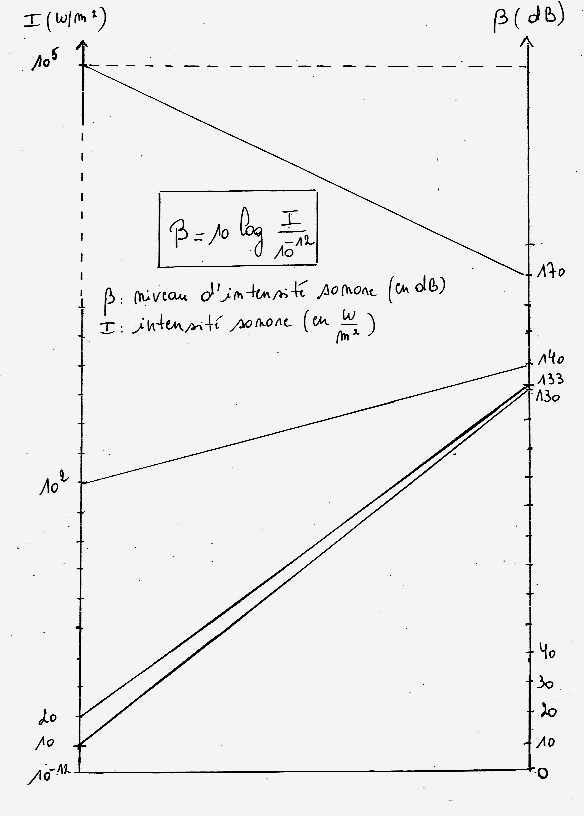
\includegraphics[width=10.269cm,height=14.349cm]{Pictures/10000001000002480000033056ED2EA613E32604.png}\emph{\textbf{Exercices}}

Convertir en dB, les intensités sonores de~:

\begin{enumerate}
	\item I = $10^{-12} \si{w/m^2}$ (Rép~: 0 dB)
	\item I = $10 \si{ W/m^2 }$ (Rép~: 130 dB)
        \item I = $20 \si{w/m^2}$ (Rép~: 133 dB)
	\item I = $10^{2} \si{W/m^2}$ (Rép~: 140 dB)
	\item I = $10^5 \si{w/m^2}$ (Rép~: 170 dB)
\end{enumerate}

\subsection{Exercice}

\begin{enumerate}
\item Calculez le niveau d'intensité sonore émis par un haut-parleur
produisant un son d'une intensité sonore de $10^{-5}$ \si{w/m^2}(Rép~: 70 dB)
\item Calculez le niveau d'intensité sonore émis par deux haut-parleurs
produisant chacun un son d'une intensité sonore de
10\textsuperscript{-5} \si{w/m^2}(Rép~: 73 dB)
\item Calculez le niveau d'intensité sonore émis par trois haut-parleurs
produisant chacun un son d'une intensité sonore de
10\textsuperscript{-5} \si{w/m^2}(Rép~: 75 dB)
\item Calculez le niveau d'intensité sonore émis par dix haut-parleurs
produisant chacun un son d'une intensité sonore de
10\textsuperscript{-5} \si{w/m^2}(Rép~: 80 dB)
\end{enumerate}

\subsection{Conclusion}

L'échelle des décibels n'est pas une échelle linéaire (c'est une échelle
logarithmique).

\emph{Chaque fois que l'intensité sonore double , le niveau
d'intensité sonore augmente de approximativement 3 dB}. Autrement dit,
un son deux fois plus intense verra son niveau d'intensité sonore
augmenter de 3 dB.

Si l'intensité sonore est \textbf{multipliée par 10}, le niveau
d'intensité sonore \textbf{augmente} exactement de 10 dB (car il s'agit
d'un logarithme en base 10).

\subsection{Règles
en vigueur en Belgique. }

Pour la sécurité de vos oreilles, je vous conseille vivement de lire
le livre de la page 53 à 55.

\emph{En Belgique, un arrêté de l'Exécutif régional wallon
limite à 90 dB le niveau d'intensité sonore dans les discothèques et
salles de concert}. Cette norme sécuritaire est malheureusement trop
peu souvent respectée.

Il existe une application sur les Smartphones~: le sonomètre.
Téléchargez l'application, essayer là et faites en une démonstration en classe si vous le désirez.

\subsection{Exercices}

\subsubsection{Exercice 1}
 Calculer le niveau d'intensité sonore correspondant à un ensemble de
trois sources identiques produisant chacune séparément un niveau
d'intensité sonore de 60 dB.

\subsubsection{Exercice 2}

Dans une pièce, une imprimante produit un son d'un niveau sonore de
60 dB. Simultanément, dans la même pièce, un ventilateur produit un son
de niveau sonre égal à 50 dB. Calculer le niveau d'intensité sonore
perçu par un auditeur dans la pièce.

\subsubsection{Exercice 3}

Un son de niveau d'intensité sonore de 70 dB atteint un mur dans
lequel il perd 99\% de son intensité en le traversant. Quel est le
niveau d'intensité sonore perçu après avoir traversé le mur~? (C'est à
peu près ce qu'il se passe entre deux locaux dans lesquels deux profs
donnent cours en parlant simultanément).

\subsubsection{Exercice 4}
En Belgique, l'exposition des travailleurs à des bruits de niveau
d'intensité sonore de 80 dB pendant 8 heures par jour est considérée
légalement comme le plafond à ne pas dépasser. Pour un niveau
d'intensité sonore de seulement 3 dB en plus, la durée d'exposition doit
être réduite de moitié, soit 4 heures maximum. Justifie la logique de
cette règle.

\subsubsection{Exercice 5}
 Une exposition quotidienne durant 8 heures à un niveau d'intensité
sonore de 80 dB est considérée par la loi belge comme étant la limite
maximale à ne pas dépasser.

Calculez la durée d'exposition quotidienne à ne pas dépasser si le
niveau d'intensité sonore est de 98 dB (comme dans beaucoup de
discothèques ou lorsque vous êtes proches des enceintes à un festival).

\subsubsection{Exercice 6}

Calculer le niveau d'intensité sonore correspondant à un ensemble de
trois sources identiques produisant chacune séparément un niveau
d'intensité sonore de 60 dB.

\subsubsection{Exercice 7}
Dans une pièce, une imprimante produit un son d'un niveau sonore de
60 dB. Simultanément, dans la même pièce, un ventilateur produit un son
de niveau sonre égal à 50 dB. Calculer le niveau d'intensité sonore
perçu par un auditeur dans la pièce.

\subsubsection{Exercice 8}
Un son de niveau d'intensité sonore de 70 dB atteint un mur dans
lequel il perd 99\% de son intensité en le traversant. Quel est le
niveau d'intensité sonore perçu après avoir traversé le mur~? (C'est à
peu près ce qu'il se passe entre deux locaux dans lesquels deux profs
donnent cours en parlant simultanément).

\subsubsection{Exercice 9}
En Belgique, l'exposition des travailleurs à des bruits de niveau
d'intensité sonore de 80 dB pendant 8 heures par jour est considérée
légalement comme le plafond à ne pas dépasser. Pour un niveau
d'intensité sonore de seulement 3 dB en plus, la durée d'exposition doit
être réduite de moitié, soit 4 heures maximum. Justifie la logique de
cette règle.

\subsubsection{Exercice 10}
Une exposition quotidienne durant 8 heures à un niveau d'intensité
sonore de 80 dB est considérée par la loi belge comme étant la limite
maximale à ne pas dépasser.

Calculez la durée d'exposition quotidienne à ne pas dépasser si le
niveau d'intensité sonore est de 98 dB (comme dans beaucoup de
discothèques ou lorsque vous êtes proches des enceintes à un festival).

\subsection{Intensité à une distance  d'une source isotrope }

Imaginez une source, l'explosion d'un pétard par exemple, qui produit un
son d'une certaine puissance P. Pourrions-nous calculer l'intensité
sonore perçue si vous êtes à une certaine distance R du pétard~?

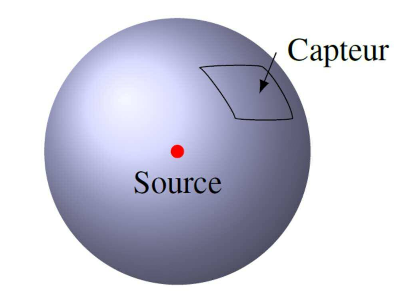
\includegraphics[width=7.103cm,height=5.315cm]{Pictures/100000010000018C00000128C1F2235D9C61A7FD.png}Imaginons
que l'on soit à une certaine distance R d'une source qui émet une
énergie E pendant un temps t. Ici, l'énergie est émise également dans
toutes les directions, ce qui signifie qu'on a affaire à une source
isotrope.

Ainsi, à une certaine distance r, l'énergie émise est distribuée
également sur une sphère entourant la source.

À une certaine distance de la source, il y a un capteur ayant une aire
$A_{\mbox{capteur}}$. Le capteur ne capte qu'une partie de l'énergie émise par la
source.

La proportion captée est donnée simplement par le rapport entre l'aire
du capteur ($A_{\mbox{capteur}}$) et l'aire totale sur laquelle est répartie
l'énergie de la source.

\subsection{Exercices}

\subsubsection{Exercice 11}

Une source lumineuse isotrope a une puissance de 100 \si{w}.  Quelle est l'intensité sonore de l'onde captée à 120 \si{m} de la source?

\subsubsection{Exercice 12}
Une personne crie à 100 m de distance d'un auditeur en produisant un son
d'une intensité perçue de 55 dB. Quelle sera le niveau d'intensité
sonore perçu par cet auditeur si 20 000 personnes se trouvant à 100 m de
distance de cet auditeur produisent chacune un cri identique ?

\subsubsection{Exercice 13}
Un auditeur se trouvant à 50 mètres de distance d'une source sonore
isotrope capte un son de 100 dB. Quel est le niveau d'intensité sonore
perçu par l'auditeur à 1 km de distance de la source?

\subsubsection{Exercice 14}
L'explosion d'un pétard produit un son ayant une intensité de 40 dB
quand on est à 50 m du pétard. Quelle est l'intensité (en dB) du son
produit par l'explosion de 1000 pétards si on est à 200 m de
l'explosion?
